\section{Setup}
For the use case implementation different sensors, actors and software packages were developed. This section covers the respective use of each sensor, actor and software package. Some software packages will be at a later point in time to match the different edge computing platforms. But the core functionality while remain for each software package.

\subsection{Compute units}\label{subsec:compute-units}
For this experiment, up to three Raspberry Pi's and one external \gls{tpu} are available. The chosen \textit{Raspberry Pi 4 Model B} is equipped with 4 GB of \gls{RAM}. The Raspberry Pi's are referred to as nodes of the edge computing system. Each node is powered by \gls{PoE}. Each node has an official Raspberry Pi \gls{PoE} hat mounted on top. Also, each node has a passive cooled enclosing. One \textit{TP-Link TL-SG1005P} 5-Port Gigabit PoE Switch provides the power and the connection to the router. Each node is connected to the switch via a \textit{CAT 6} network cable. For connecting the sensor to the system, an WiFi \gls{AP} is provided. Figure \ref{fig:network-topology} shows the overall network topology of the three nodes.

\begin{figure}[H]
    \fontsize{9}{10}\selectfont % <-- adjust font in svg
    \centering
    \def\svgwidth{\textwidth}
    \input{assets/setup/compute-units_wiring.drawio.pdf_tex}
    \caption{Network topology.}
    \label{fig:network-topology}
\end{figure}

The network has an internal and external bandwidth bottleneck. The internal bottleneck refers to the connection between the router and the first switch, which is limited to 1 Gbit/s. The external bottleneck is limited by the booked data usage plan of 100 Mbit/s. These bottlenecks then results in an internet download bandwidth of 100 Mbit/s and an internal data transfer rate of 1 Gbit/s.

\bigskip
It should be noted the software packages which will run on the edge computing platforms need to be cross compiled to match the Raspberry Pi's processor architecture. Each Raspberry Pi comes with a quad-core \textit{Cortex-A72 (ARM v8)} processor \cite{Raspberrypifoundation}. Due to the fact that the used processors in this experiment are ARM based (\ref{subsec:compute-units}) the container images or any other executable must be compiled to run on ARM devices. To be more clearly, the cross compile target platform is `linux/arm64/v8` for the Raspberry Pi's running Ubuntu 20.04 ARM in 64 Bit.


\subsection{BMP 280 Sensor}\label{subsec:bmp280}
The BMP 280 is a sensor which provides environmental data like temperature, pressure and altitude over I2C or SPI \cite{Az-delivery-BMP280}. The following setup explains how the sensor device for temperature, pressure and altitude was implemented. Next to the BMP 280 the microcontroller ESP32 Dev Kit C V4 was used to read and transfer the data via MQTT to the nearby edge computing platform. The application, running on the ESP32, was build inside Microsoft’s Visual Studio Code editor in conjunction with the PlatformIO extension. For simplification purposes the initial application was generated, configured and implemented inside a PlatformIO project. PlatformIO provides developers with tools to write applications for embedded products in a cross-platform, cross-architecture and multiple framework way \cite{Platformio}. The software for gathering and sending the data to the edge platform uses the Arduino framework. 

\bigskip
For talking to the BMP 280 sensor the C++ library from Adafruit \cite{Adafruit} was used. The used BMP 280 sensor from AZ-Delivery is only partially compatible to the Adafruit BMP 280 library \cite{Az-delivery-BMP280}. To work correctly the I2C address had to be changed to 0x76 instead of 0x77 in the header file.
 
\bigskip
The following figure \ref{fig:wiring-bmp280} shows the wiring of the BMP 280 to the ESP32 microcontroller. The wiring also includes LEDs which visually presents the connection status of the ESP32 to the Wi-Fi network and to the programmed MQTT broker. Figure \ref{fig:bmp280} show the wiring of Figure \ref{fig:wiring-bmp280} twice in real life.

\begin{figure}[H]
    \centering
    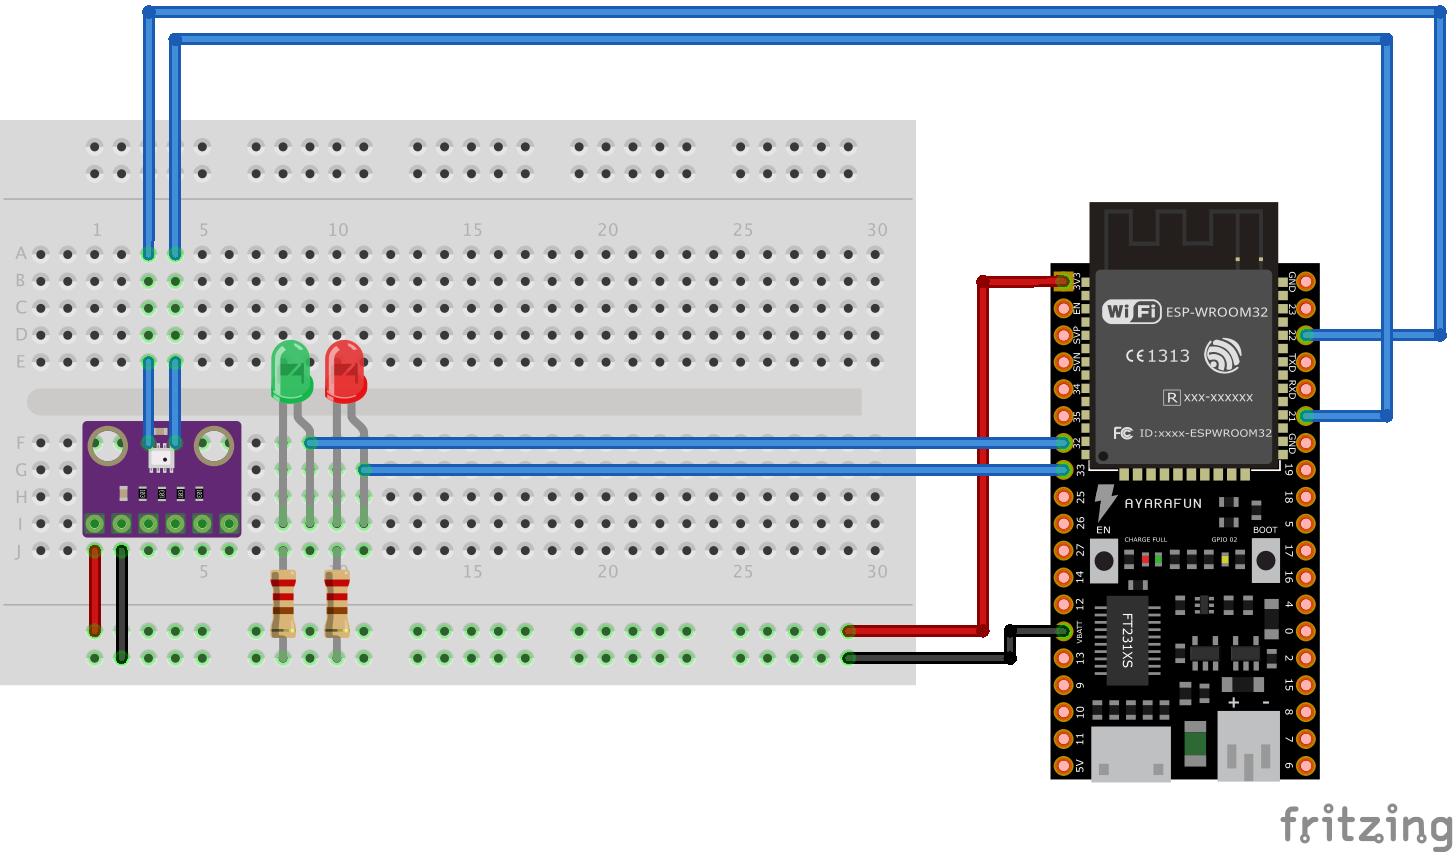
\includegraphics[width=\textwidth]{assets/setup/wiring-bmp280.png}
    \caption{BMP 280 wiring to the ESP32.}\label{fig:wiring-bmp280}
\end{figure}

\begin{figure}[H]
    \centering
    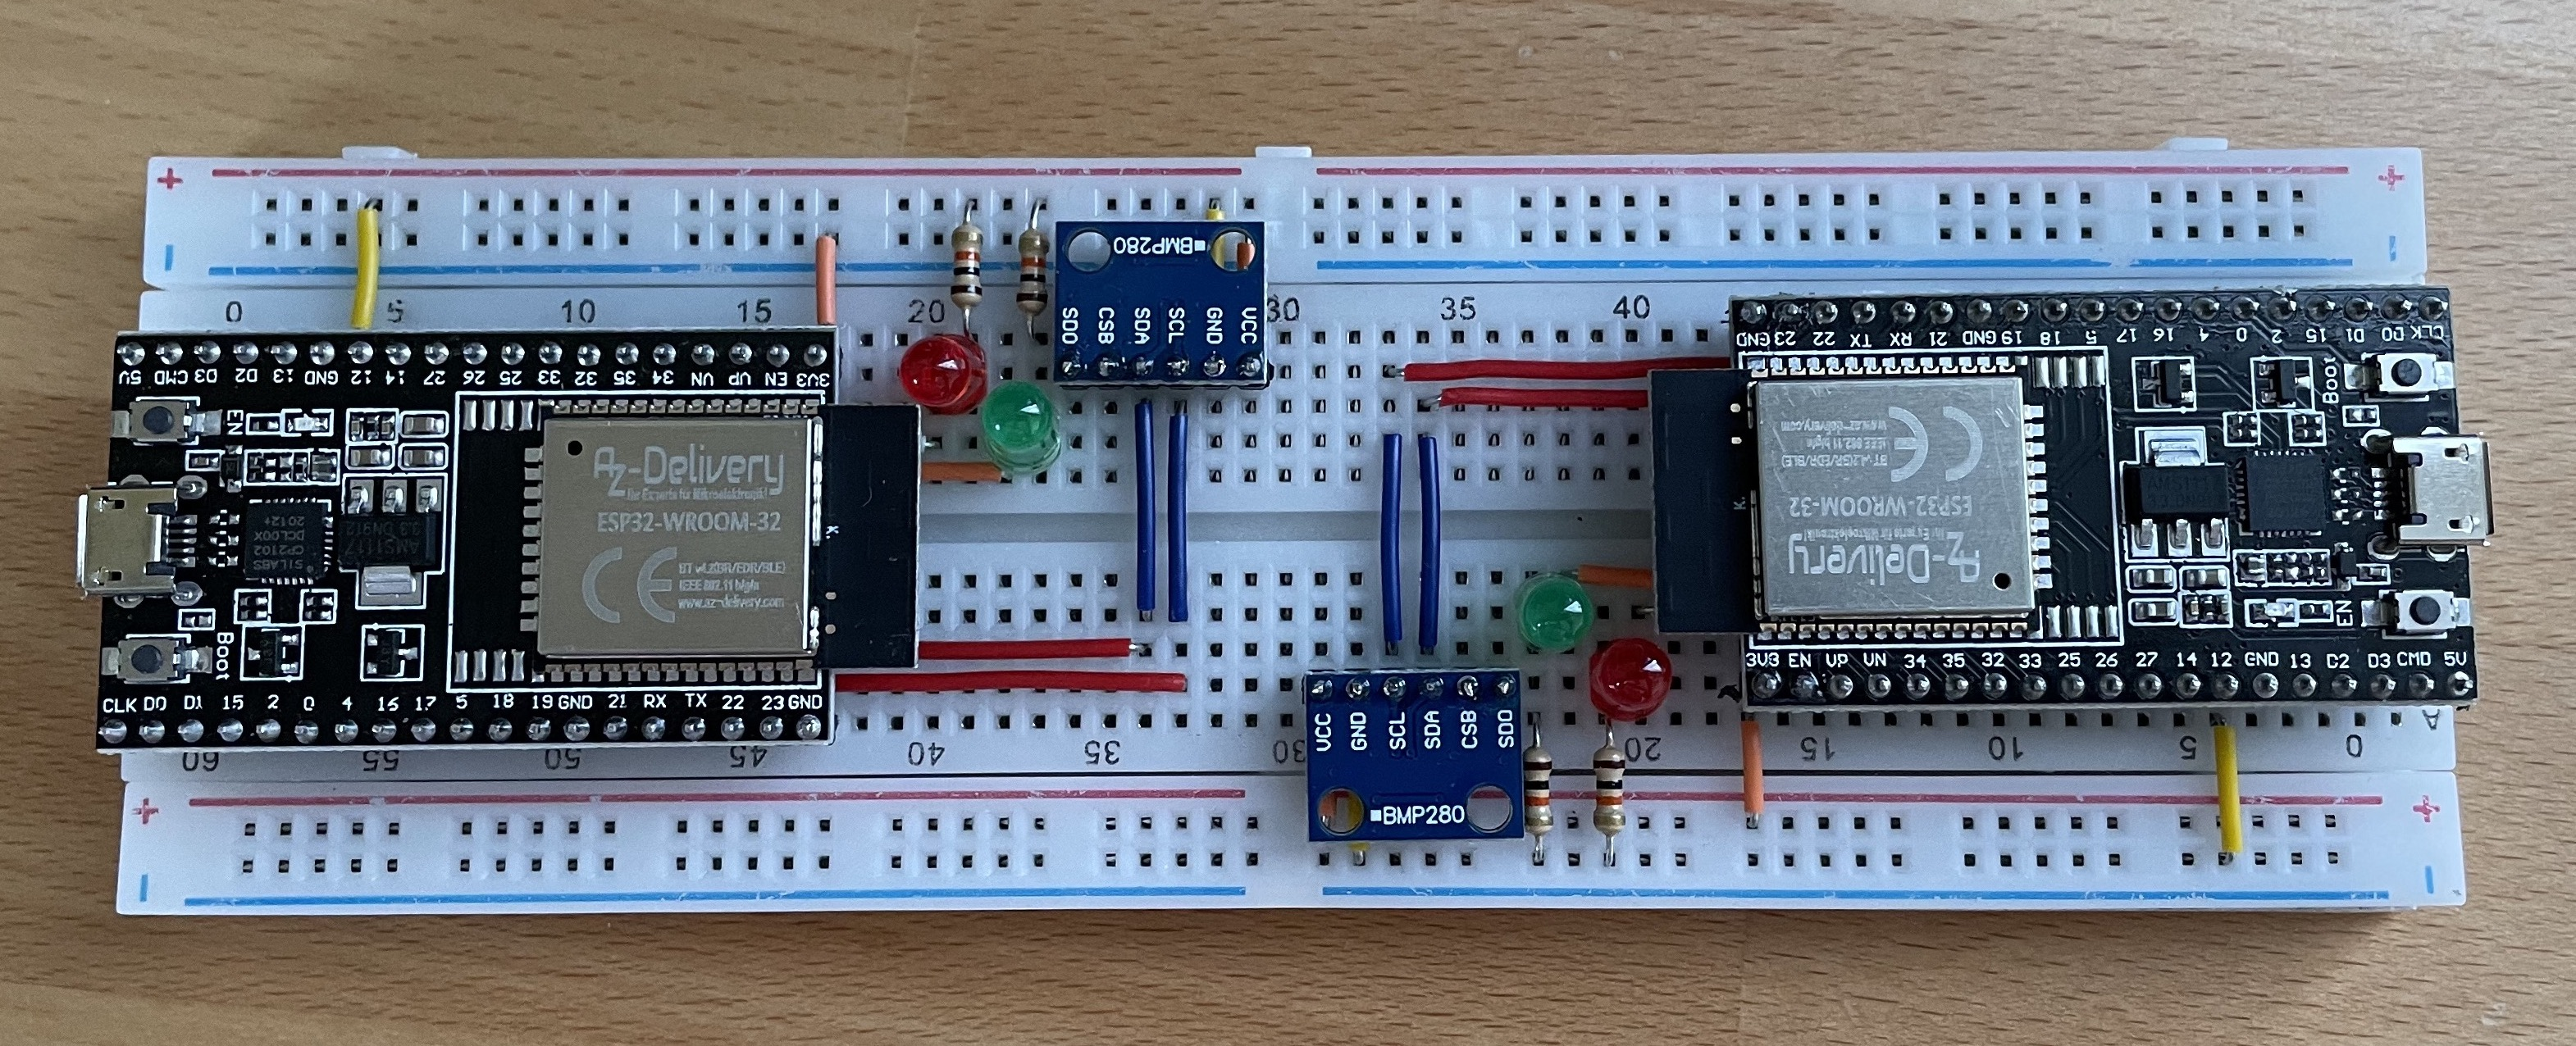
\includegraphics[width=\textwidth]{assets/setup/bmp280.jpeg}
    \caption{Real breadboard of two BMP 280 wired to their ESP32.}\label{fig:bmp280}
\end{figure}


\subsection{MQ-2 gas sensor}\label{subsec:mq2}
The MQ-2 is a sensor which detects LPG, i-butane, propane, methane, alcohol, hydrogen and smoke in the surrounding environment \cite{Az-delivery-MQ-2}. The following setup explains how the sensor device was implemented. Next to the MQ-2 the microcontroller ESP32 Dev Kit C V4 was used to read and transfer the data via MQTT to the nearby edge computing platform. The application, running on the ESP32, was built with the same tools as the BMP280 sensor (VS Code Editor and PlatformIO).

\bigskip
For talking to the MQ-2 sensor no library is required. The microcontroller only needs to read one digital and one analog pin. The digital pin provides information about whether gas is in the sensor environment or not. The analog pin returns a percentage value of the gas in the air.

\bigskip
The following figure \ref{fig:wiring-mq-2} shows the wiring of the MQ-2 sensor to the ESP32 microcontroller. Figure \ref{fig:mq-2} show the above wiring of Figure \ref{fig:wiring-mq-2} twice in real life.

\begin{figure}[H]
    \centering
    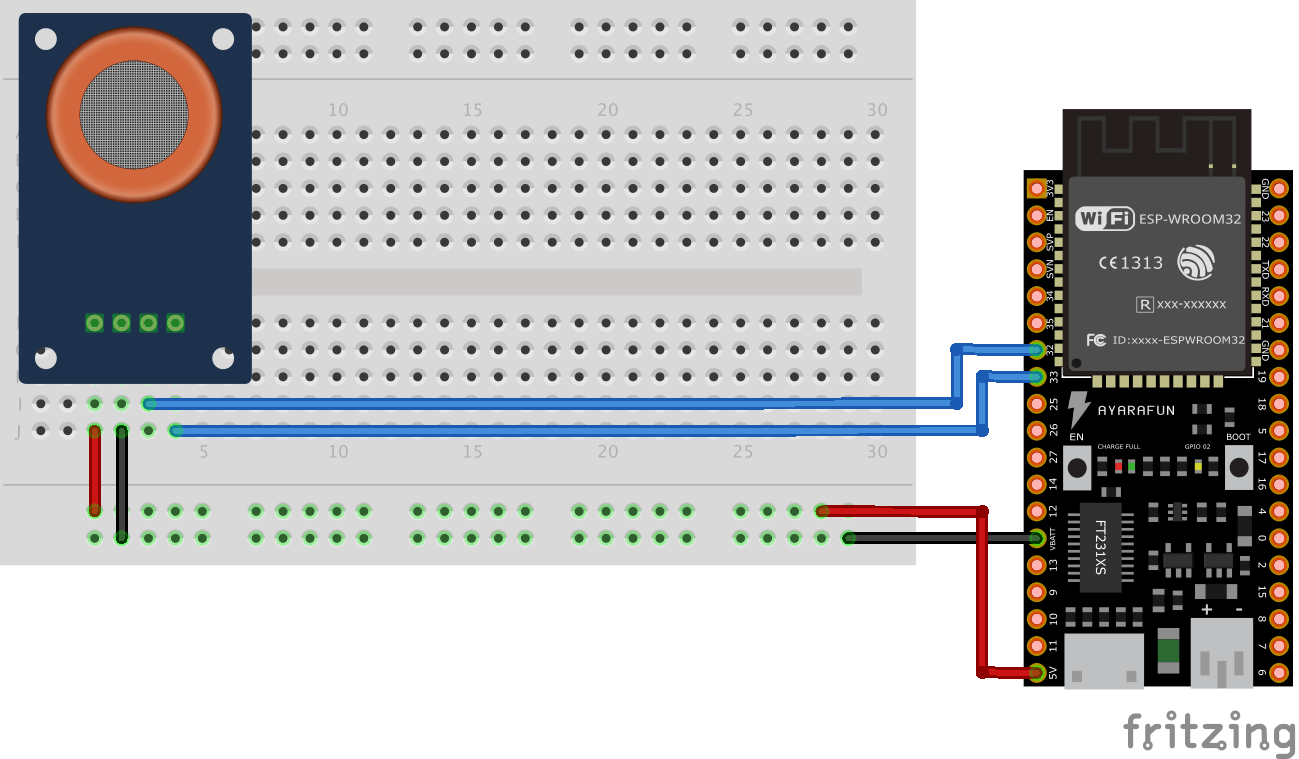
\includegraphics[width=\textwidth]{assets/setup/wiring-mq-2.png}
    \caption{BMP 280 wiring to the ESP32}\label{fig:wiring-mq-2}
\end{figure}

\begin{figure}[H]
    \centering
    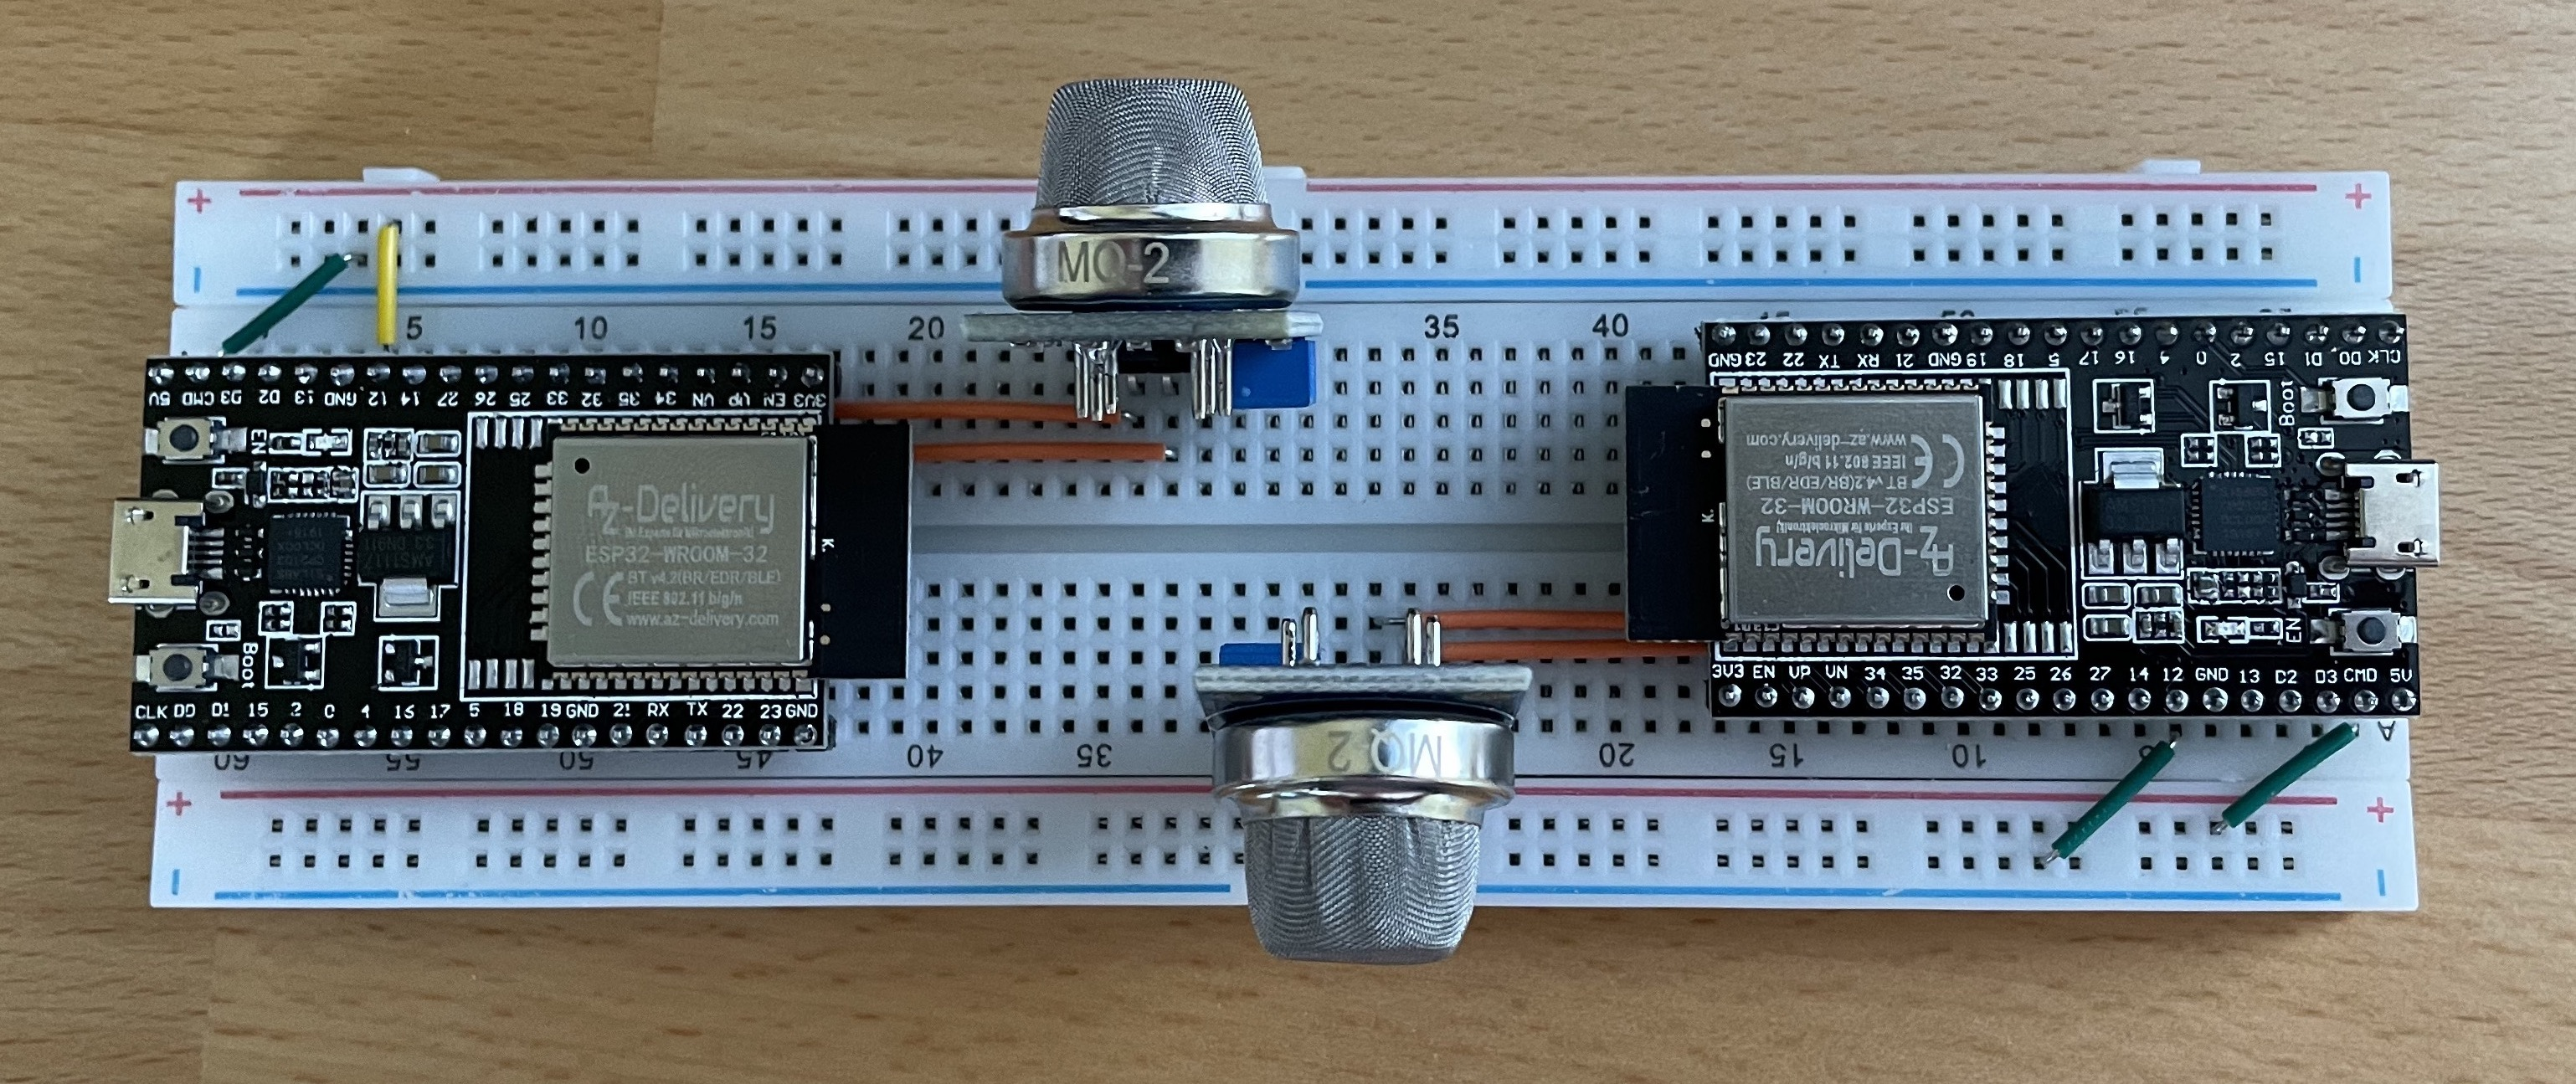
\includegraphics[width=\textwidth]{assets/setup/mq-2.jpeg}
    \caption{Real breadboard of two BMP 280 wired to their ESP32.}\label{fig:mq-2}
\end{figure}

Its also worth noting the MQ-2 sensor must settle for some time until credible data is generated. Figure \ref{fig:mq-2-percent-drop} shows the drop on gas percentage in the air over 30mins.

\begin{figure}[H]
    \centering
    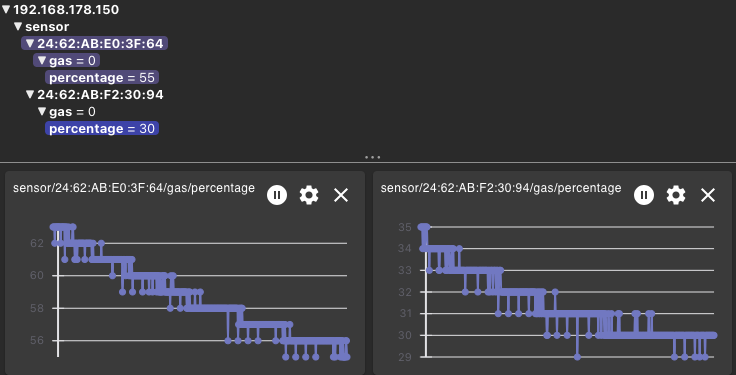
\includegraphics[width=\textwidth]{assets/setup/mq-2-percent-drop.png}
    \caption{Gas percentage drop over a 30min period.}\label{fig:mq-2-percent-drop}
\end{figure}


\subsection{Ventilation control}\label{subsec:ventilation}
This simple device controls a ventilation for venting in the event of the occurrence of hazardous gases or high temperature. This device does not detect the gas itself it just controls the ventilator. The used, two pin, ventilator model YDL3007C05 can be operated between 3.3V and 5V which is optimal to directly attach it to a microcontroller like an ESP32 or ESP8266. For this project an NodeMCU Lolin V3 Module ESP8266 ESP-12F \cite{Az-delivery-ESP8266} was used to start and stop the ventilator accordingly to the published states from a configured MQTT broker.

\bigskip
The application, running on the ESP8266, was built with the same tools as the devices described in previous sections (VS Code Editor and PlatformIO). The used framework was also the Arduino framework. For controlling the ventilator no specific library is required. The microcontroller only needs to set one GPIO pin to high for on or low for off.

\bigskip
The following figure \ref{fig:wiring-ventilator} shows the wiring of the ventilator to the ESP8266 microcontroller. Figure \ref{fig:ventilator} show the above wiring of Figure \ref{fig:wiring-ventilator} in real life.

\begin{figure}[H]
    \centering
    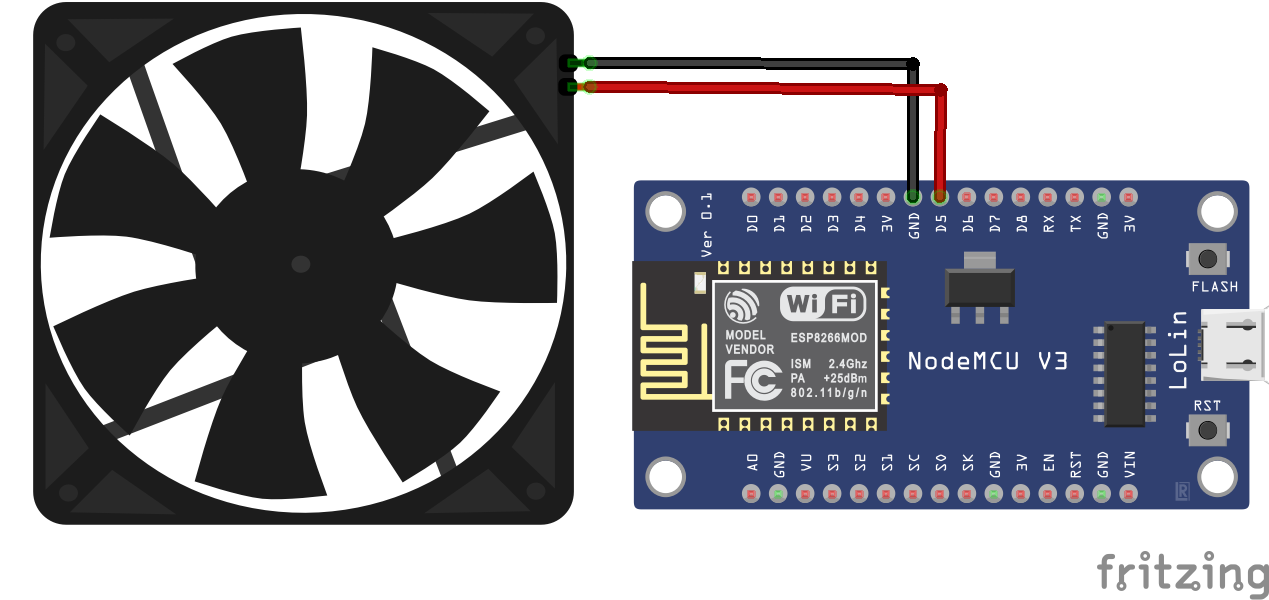
\includegraphics[width=\textwidth]{assets/setup/wiring-ventilator.png}
    \caption{Ventilator wiring to the ESP8266.}\label{fig:wiring-ventilator}
\end{figure}

\begin{figure}[H]
    \centering
    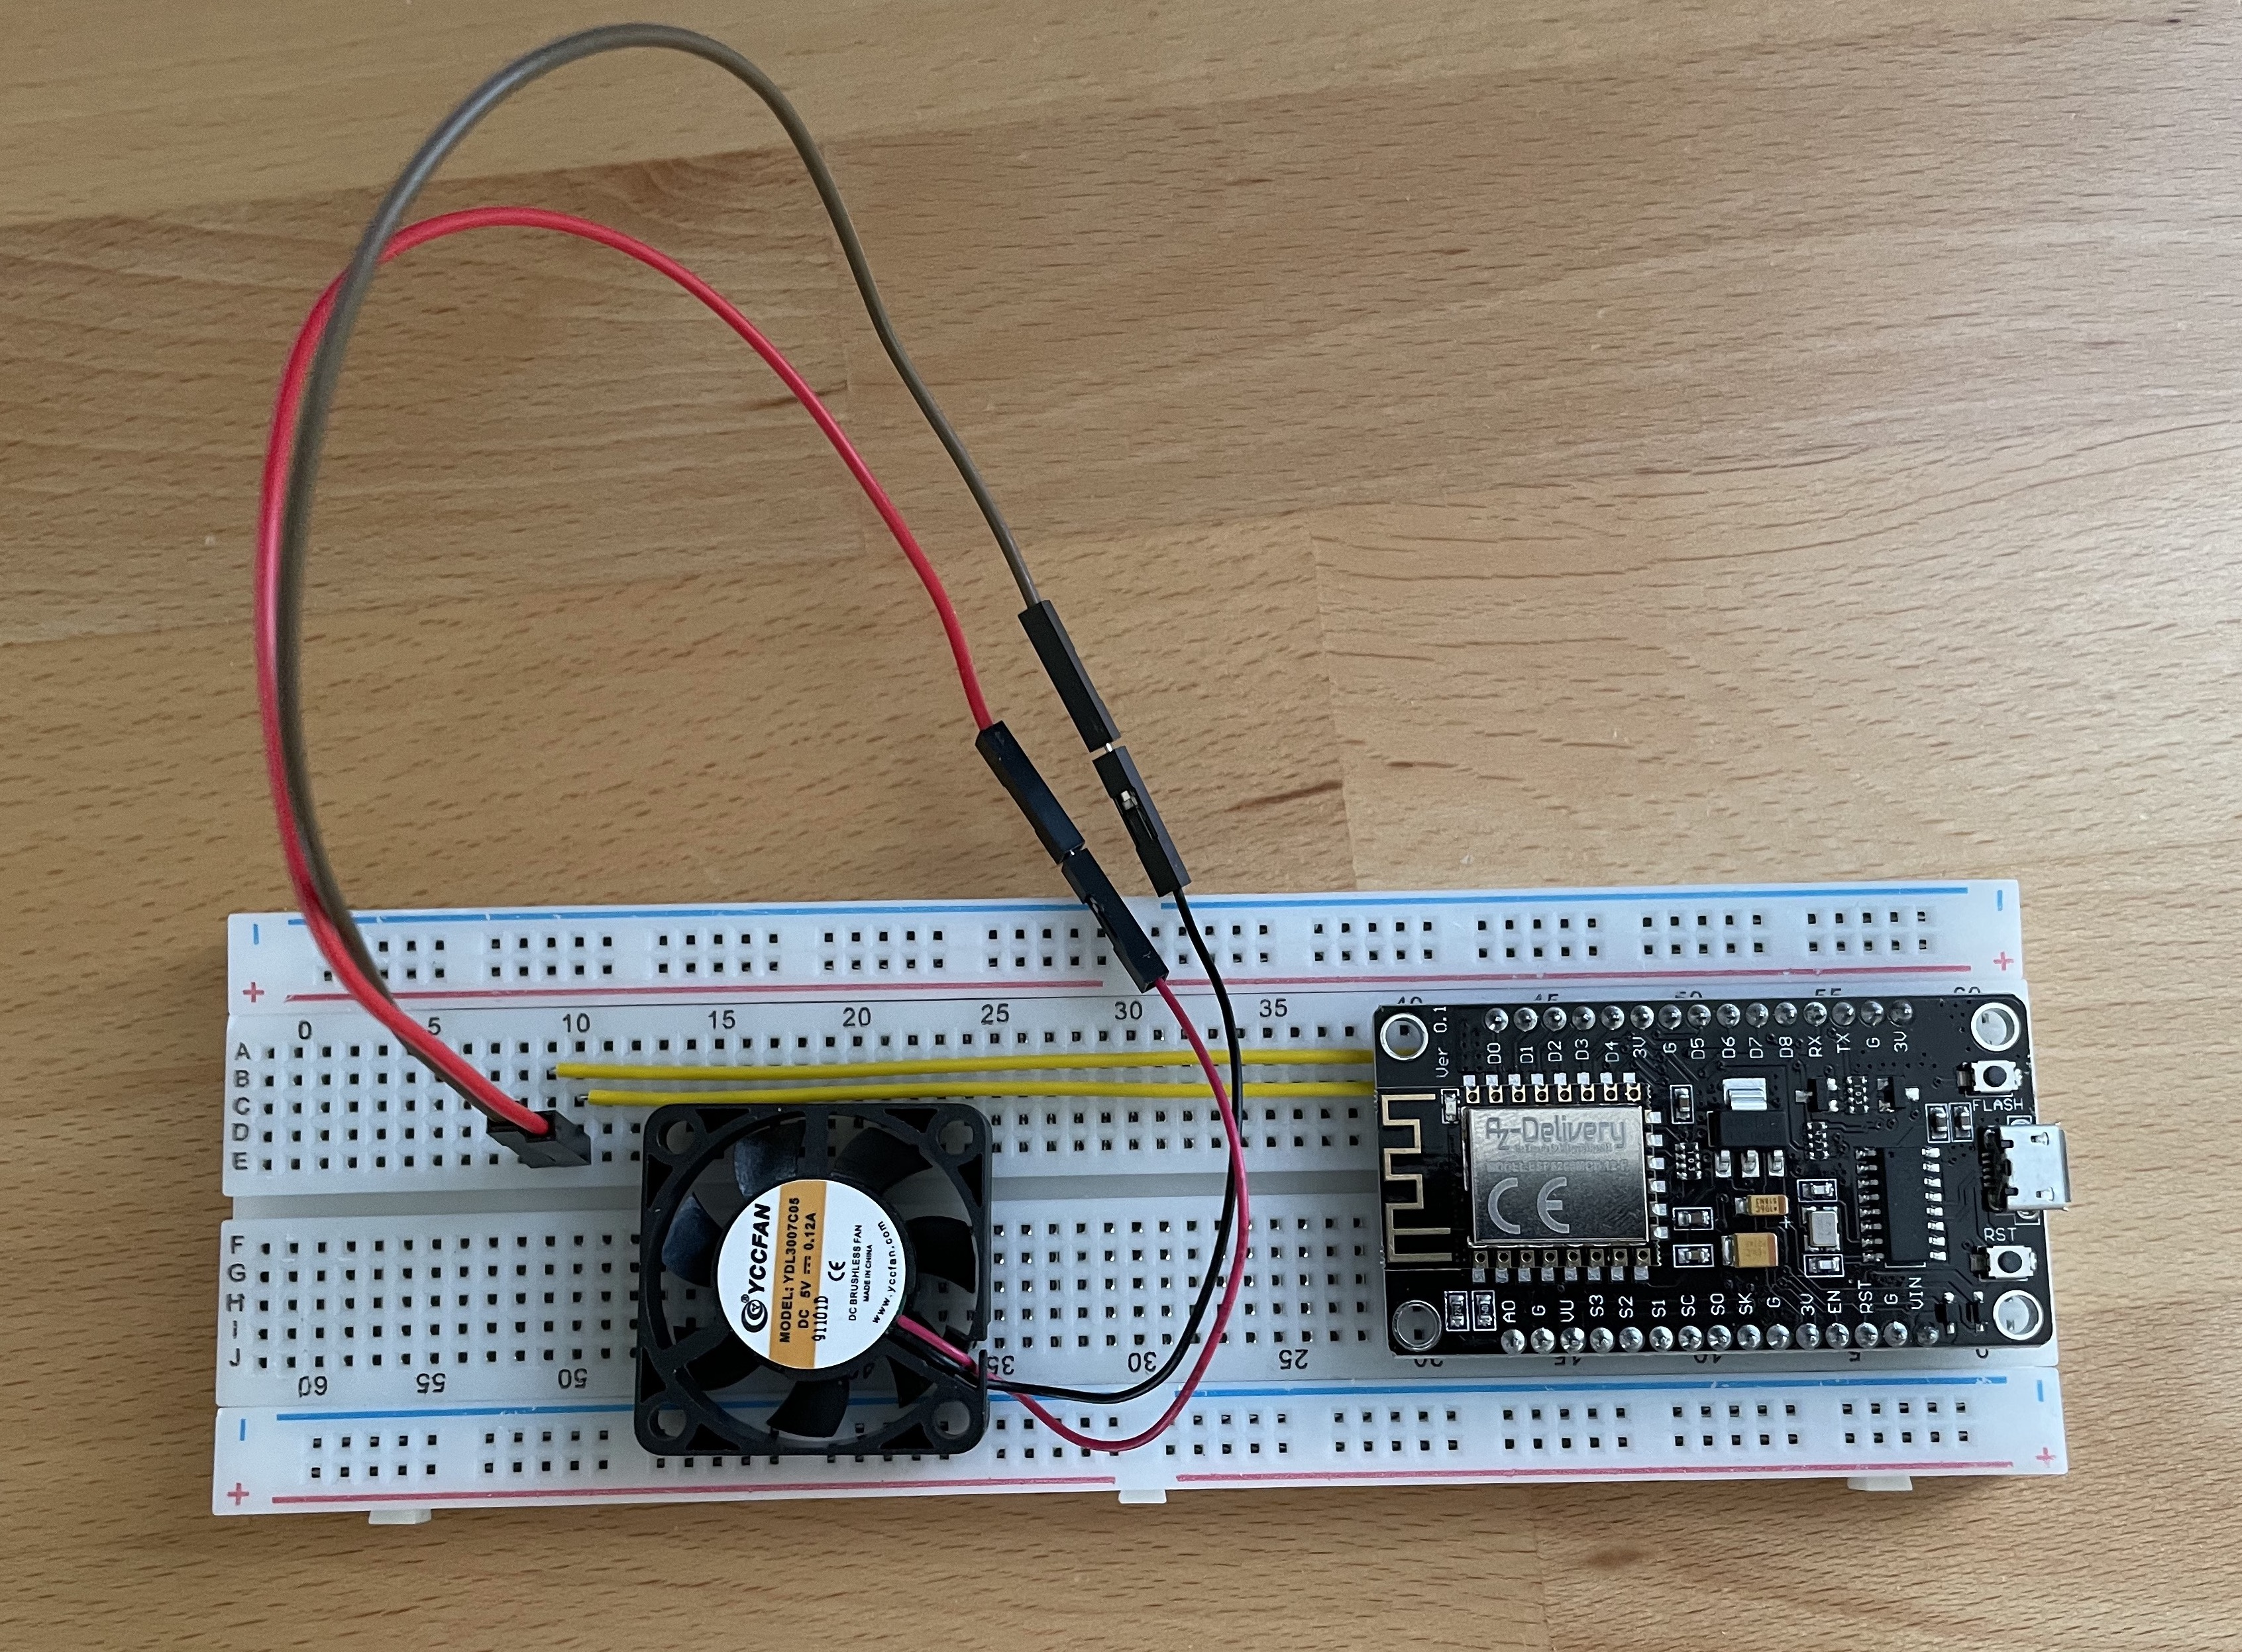
\includegraphics[width=\textwidth]{assets/setup/ventilator.jpeg}
    \caption{Real breadboard of ventilator wired to its ESP8266.}\label{fig:ventilator}
\end{figure}


\subsection{Camera sensor}\label{subsec:camera-sensor}
The setup also includes a camera that captures images for later processing with machine learning models (processing in section \ref{subsec:detector-service}). The camera sensor is represented as a combination of the official PiCamera and a Raspberry Pi 3B+. The python program, running on the Raspberry Pi, takes pictures in a predefined period and encodes them to a base64 string. The encoded string is then published to a given topic inside the MQTT broker of the connected edge platform for further processing by other services inside the system (see \ref{subsec:detector-service}).

%%%%%%%%%%%%%%%%%%%%%%%%%%%%%%%%%%%%%%%%%%%%%%%%%%%%%%%%%%%%%%%%%%%%%%%%%%%%%%%%%%%%%%%%%%%%%%%
% Services
%%%%%%%%%%%%%%%%%%%%%%%%%%%%%%%%%%%%%%%%%%%%%%%%%%%%%%%%%%%%%%%%%%%%%%%%%%%%%%%%%%%%%%%%%%%%%%%
\subsection{Detector service}\label{subsec:detector-service}
Detector is a service that further processes the data provided by the camera sensor of section \ref{subsec:camera-sensor}. The special feature of this service is the processing of the data by a \gls{tpu}. This \gls{tpu} is a piece of additional hardware attached via \gls{usb} to one of the nodes. The camera detection service is a small Python program which runs a MQTT client for subscribing to the corresponding topic. Received messages on the subscribed topic will then be base64 decoded and subsequently passed to the image detection, which runs a machine learning model (TensorFlow Lite model) on the attached \gls{tpu}. Results from the machine learning inference will then be published back into the system via an MQTT topic. For simplicity, an already trained model is used. The used model is a Mobile net v2 which detects different kinds of parrots. This model can be replaced with any image recognition model in the TensorFlow Lite format.

\subsection{Emergency service}\label{subsec:emergency-service}
The emergency service has the responsibility to avoid hazards regarding fire, explosions or high temperature. By monitoring the values of the BMP280 and MQ2 sensors the service will initiate countermeasures on any sign of gas or high temperature. To accomplish this the service will subscribe to the corresponding MQTT topics of the BMP280 and MQ2. Each new value is assessed for a potential hazard. For simplification reason, the only countermeasure which can be activated is the ventilation system. The ventilation system is also controlled over the MQTT protocol. The service also stores information about ongoing countermeasures in a database to prevent early shutdowns of a countermeasures.

\subsection{Database service}\label{subsec:database-service}
The database service is a service that is responsible to securely store collected data for future processing or reports in a later state. The database service should be filled with the values from both sensors, BMP280 (\ref{subsec:bmp280}) and MQ2 (\ref{subsec:mq2}). By subscribing to the corresponding MQTT topics the database can consume and store the incoming values inside a database.

\subsection{Monitoring service}\label{subsec:monitoring-service}
Monitoring will provide different kind of stats of the underlying edge computing platform. This service should be responsible to collect all the necessary data, store them and visualize them in a web frontend. The value collector can vary on each platform. For the user interface any kind of web application is possible. The user interface should present the previously collected in an appealing way like showing charts or anything similar. Example values would be the state of each node and their corresponding CPU and memory utilization.
